\chapter{Results and Analysis}
\label{chapter:results}
For our first research question, we regress \ac{ei} on the three independent variables proposed by Ajzen's \ac{tpb}. As shown in Table \ref{ANOVA}, we find that the explanatory power of the variables proposed by Ajzen is high (F=91.18, p<.01). The statistical analysis of the individual explanatory variables partially supports Ajzen's \ac{tpb} (see: Table \ref{Coefficients}). \ac{atb} is positively and significantly related to \ac{ei} (b=.771, p<.01). This supports our first hypothesis 1a. Hypotheses 1b suggests that \ac{sn} positively influence \ac{ei}. Our data does not provide evidence for this hypothesis. However, \ac{sn} exhibits a significant bivariate correlation with \ac{ei} (r=.449, p<.01). Furthermore, \ac{ei} was positively and significantly predicted by \ac{pbc} (b=.249, p<.01). Thus, our findings support H1c.

\begin{table}[H]
\centering
\caption{ANOVA}
\label{ANOVA}
\begin{tabular}{@{}llllll@{}}
\toprule
            & Sum of squared errors & df & Mean square & F & Sig. \\ \midrule
Regression & 150.45 & 3 & 50.15  & 91.18             & ***            \\
Residual & 34.10  & 62 & .55  &            &        \\
Total & 184.56  & 65 &    &              &              \\ \bottomrule 
\end{tabular}
\end{table} 

\begin{table}[H]
\centering
\caption{Coefficients: \ac{ei} $\sim$ \ac{atb} + \ac{sn} + \ac{pbc}}
\label{Coefficients}
\begin{tabular}{@{}llllll@{}}
\toprule
            & Estimate & Std. error & t value & Pr(\textgreater|t|) & Signif. code \\ \midrule
(Intercept) & -0.869 & 0.359    & -2.420  & 0.018             & *            \\
\ac{atb}          & 0.771  & 0.076    & 10.102  & <.001            & ***          \\
\ac{sn}          & 0.046  & 0.074    & 0.628   & 0.532             &              \\
\ac{pbc}         &  0.249  &  0.086    & 2.902   & 0.005             & **           \\ \bottomrule
\end{tabular}
\end{table}
\begin{center}
\begin{footnotesize}
Signif. codes:  0 '***' 0.001 '**' 0.01 '*' 0.05 '.' 0.1 ' ' 1
\end{footnotesize}
\end{center}

In summary, the model fits the data well. It explains 90.3\% of the variance, with adjusted R-squared being 80.6\%. Figure 4.1-4.3 illustrate the correlation of the three components of Ajzen's \ac{tpb} with the \ac{ei}.  

\begin{figure}[H]
\centering{
\caption{\ac{ei} $\sim$ \ac{atb}}
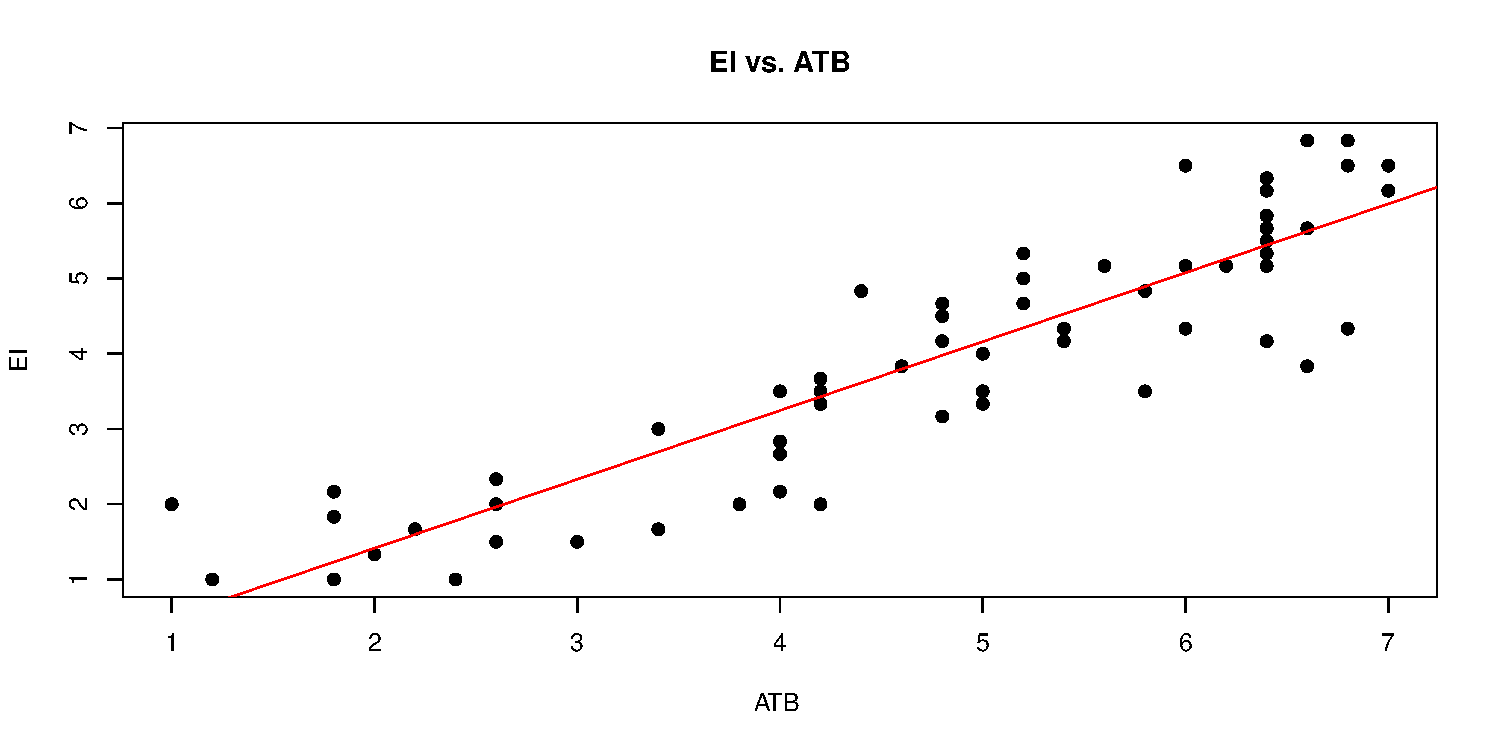
\includegraphics[width=.8\textwidth,keepaspectratio]{images/EIvsATB.pdf}}
\end{figure}

\begin{figure}[H]
\centering{
\caption{\ac{ei} $\sim$ \ac{sn}}
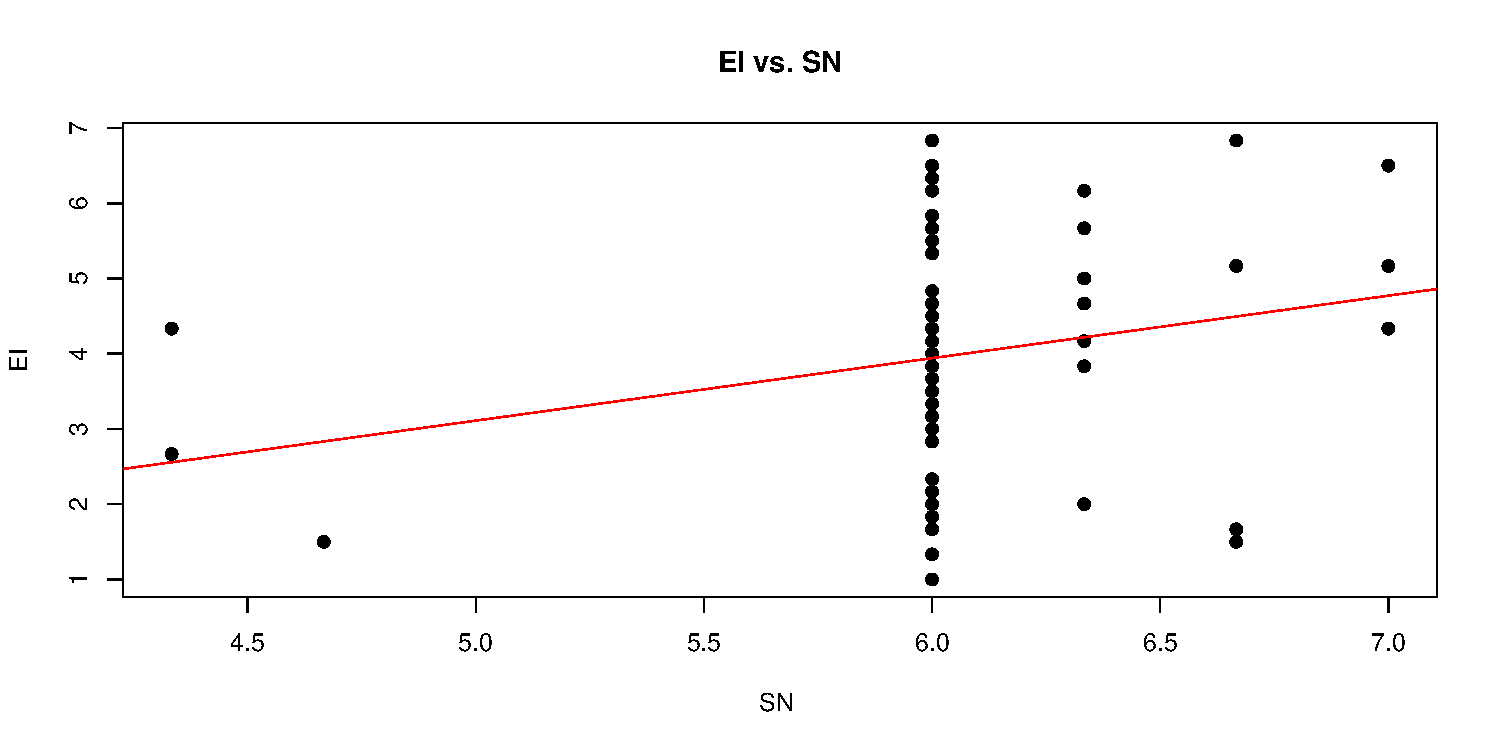
\includegraphics[width=.8\textwidth,keepaspectratio]{images/EIvsSN.pdf}}
\end{figure}

\begin{figure}[H]
\centering{
\caption{\ac{ei} $\sim$ \ac{pbc}}
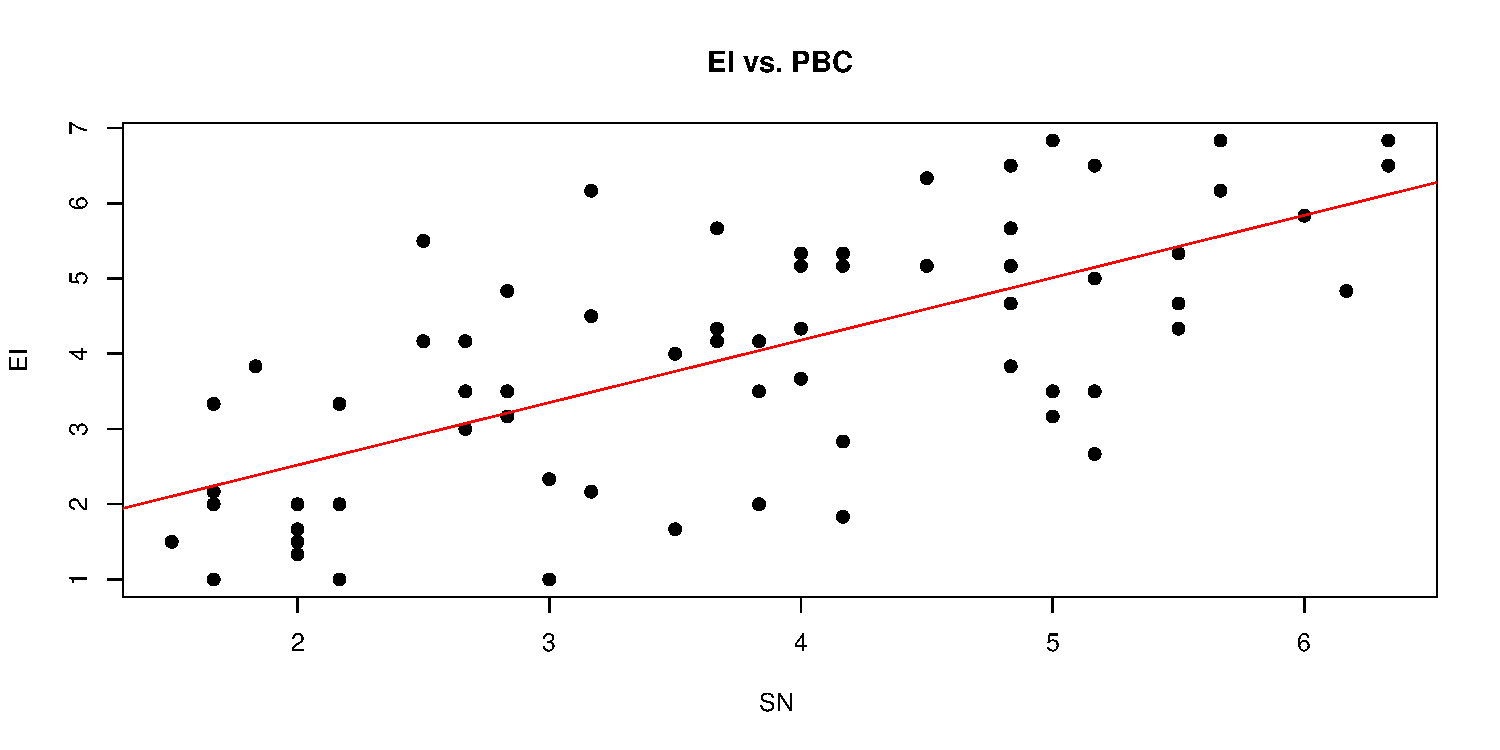
\includegraphics[width=.8\textwidth,keepaspectratio]{images/EIvsPBC.pdf}}
\end{figure}

Our second research question aims at analyzing the effect of participating in \acp{ec} on \ac{ei} (H2) and the mediating effect of the components of Ajzen's \ac{tpb} (H3a-c). Including the \acp{ec} (\ac{seba}) as the predictor variable yields a negative, non-significant effect on \ac{ei} (b=-.122, p>.77). The results of the ANOVA are depicted in Table \ref{Coefficients}. Also the correlation matrix reveals no significant relationship between attending \acp{ec} and \ac{sn} (r=-.34, p>.78), \ac{atb} (r=.02, p>.84) and \ac{pbc} (r=.20, p>.10). These relationships are visualized in appendix \ref{app:graphs}. According to \citet{baron1986moderator}, there is no effect to be moderated since no significant total effect can be observed. Thus, the indirect effects are not tested for their significance. 

\begin{table}[H]
\centering
\caption{Coefficients: \ac{ei} $\sim $ \ac{seba}}
\label{Coefficients-SEBA-EI}
\begin{tabular}{@{}llllll@{}}
\toprule
            & Estimate & Std. error & t value & Pr(\textgreater|t|) & Signif. code \\ \midrule
(Intercept) &  4.0556 & 0.2828    & 14.339   & <2e-16             & ***            \\
SEBA         &  -0.1222  &  0.4195    & -0.291   & 0.772                 &            \\ \bottomrule
\end{tabular}
\end{table}
\begin{center}
\begin{footnotesize}
Signif. codes:  0 '***' 0.001 '**' 0.01 '*' 0.05 '.' 0.1 ' ' 1
\end{footnotesize}
\end{center}

The raw data as well as the regression analysis and outcomes are publicly available at: 

\begin{center}
\textit{https://github.com/lukasmohs/entrepreneurial-intention-analysis}
\end{center} 

%see print version of our survey in appendix: \ref{app:questionaire} and raw data as well:  \ref{app:raw-data} and visualization: \ref{app:graphs}